\documentclass{beamer} 
\usepackage{amsmath,amsthm}
\usepackage{graphicx,microtype,parskip}
\usepackage{caption,subcaption,multirow}
\usepackage{attrib}

\frenchspacing

\usetheme{default}
\usecolortheme{whale}

\setbeamertemplate{navigation symbols}{}

\setbeamercolor{title}{fg=blue,bg=white}

\setbeamercolor{block title}{fg=white,bg=gray}
\setbeamercolor{block body}{fg=black,bg=lightgray}

\setbeamercolor{block title alerted}{fg=white,bg=darkgray}
\setbeamercolor{block body alerted}{fg=black,bg=lightgray}

\usepackage{etoolbox}
\newcommand{\zerodisplayskips}{%
  \setlength{\abovedisplayskip}{0pt}%
  \setlength{\belowdisplayskip}{0pt}%
  \setlength{\abovedisplayshortskip}{0pt}%
  \setlength{\belowdisplayshortskip}{0pt}}
%\appto{\normalsize}{\zerodisplayskips}
%\appto{\small}{\zerodisplayskips}
%\appto{\footnotesize}{\zerodisplayskips}


\title{Modeling changes to the functional composition of North American mammal diveristy}
\subtitle{multi-level dynamics of a regional species pool}
\author{Peter D Smits}
\institute{Department of Integrative Biology, University of California -- Berkeley}
\titlegraphic{
  
\includegraphics[width=3cm,height=3cm,keepaspectratio=true]{figure/paleodb}
  \hspace*{0.3\paperwidth}
  
\includegraphics[width=4cm,height=4cm,keepaspectratio=true]{figure/iblogo3}
}
\date{}

\begin{document}

\begin{frame}
  \maketitle
\end{frame}


\begin{frame}
  \begin{alertblock}{Question}
    When and why are certain ecologies or functional groups enriched or depleted in a species pool?
    \begin{itemize}
      \item relative abundance as function of
        \begin{itemize}
          \item species traits
          \item environmental context
        \end{itemize}
    \end{itemize}
  \end{alertblock}
\end{frame}


\begin{frame}
  \frametitle{Eco-cube and functional groups}

  \begin{center}
    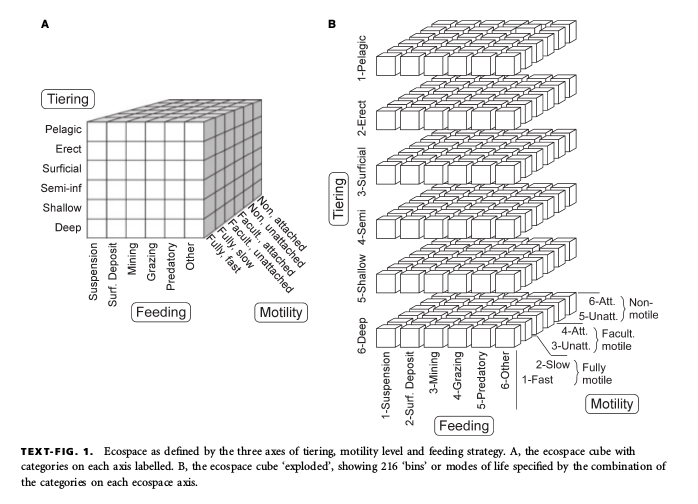
\includegraphics[height=0.8\textheight,width=\textwidth,keepaspectratio=true]{figure/ecocube}
  \end{center}

  \attrib{\footnotesize{Bambach \em{et al.}, 2007, \em{Palaeontology}}}
\end{frame}


\begin{frame}
  \frametitle{Species pool concept}

  \begin{center}
    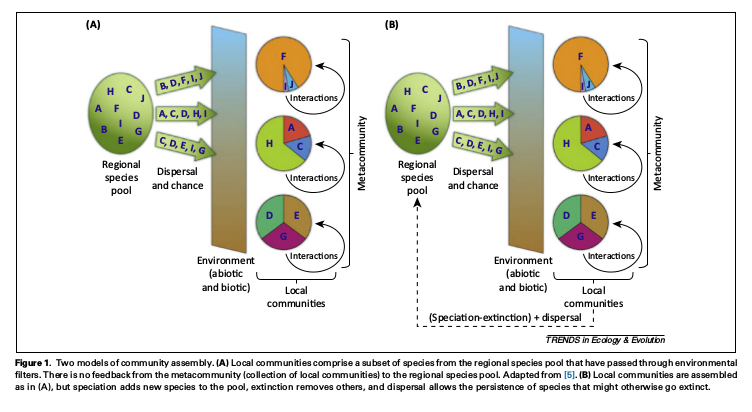
\includegraphics[height=0.8\textheight,width=\textwidth,keepaspectratio=true]{figure/schemske_pool}
  \end{center}

  \attrib{\footnotesize{Mittelbach and Schemske, 2015, \em{TREE}}}
\end{frame}

\begin{frame}
  \frametitle{Structured, multi-level data in biology}
  \begin{center}
    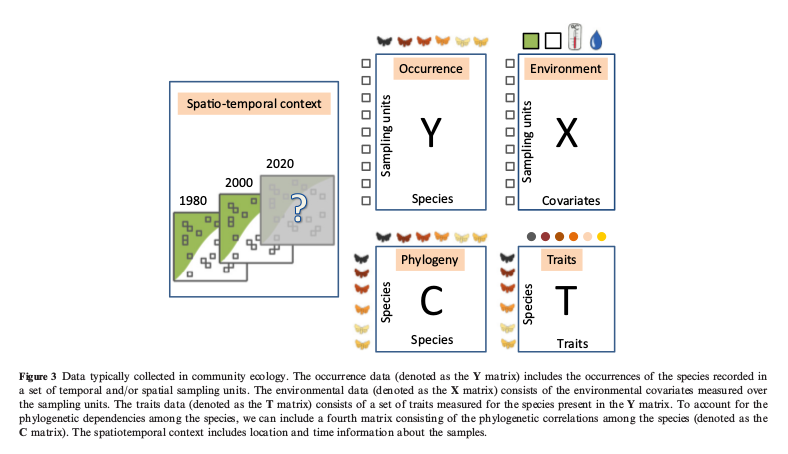
\includegraphics[width = \textwidth,height = 0.8\textheight,keepaspectratio = true]{figure/ovaskainen_data}
  \end{center}

  \tiny{\attrib{Ovaskainen \textit{et al.} 2017 \em{Ecology Letters}}}
\end{frame}

\begin{frame}
  \frametitle{Cenozoic mammals of North America}
  \begin{center}
    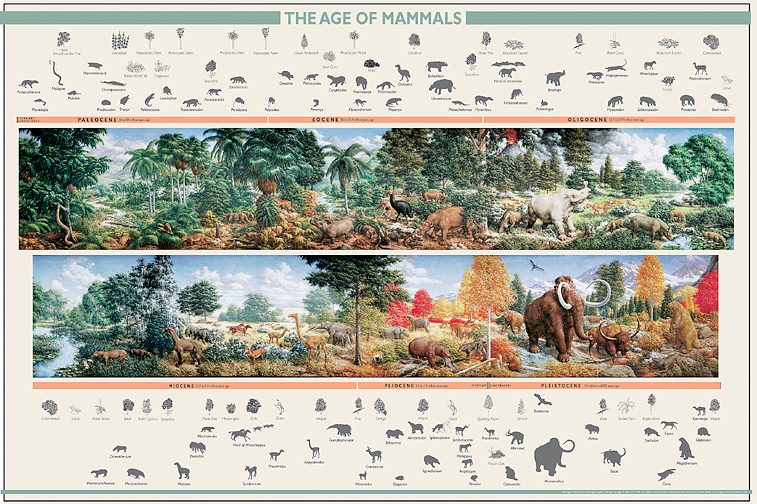
\includegraphics[height=0.8\textheight,width=\textwidth,keepaspectratio=true]{figure/aom}
  \end{center}
\end{frame}

%\begin{frame}
%  \frametitle{Differences in extinction risk}
%
%  \begin{center}
%    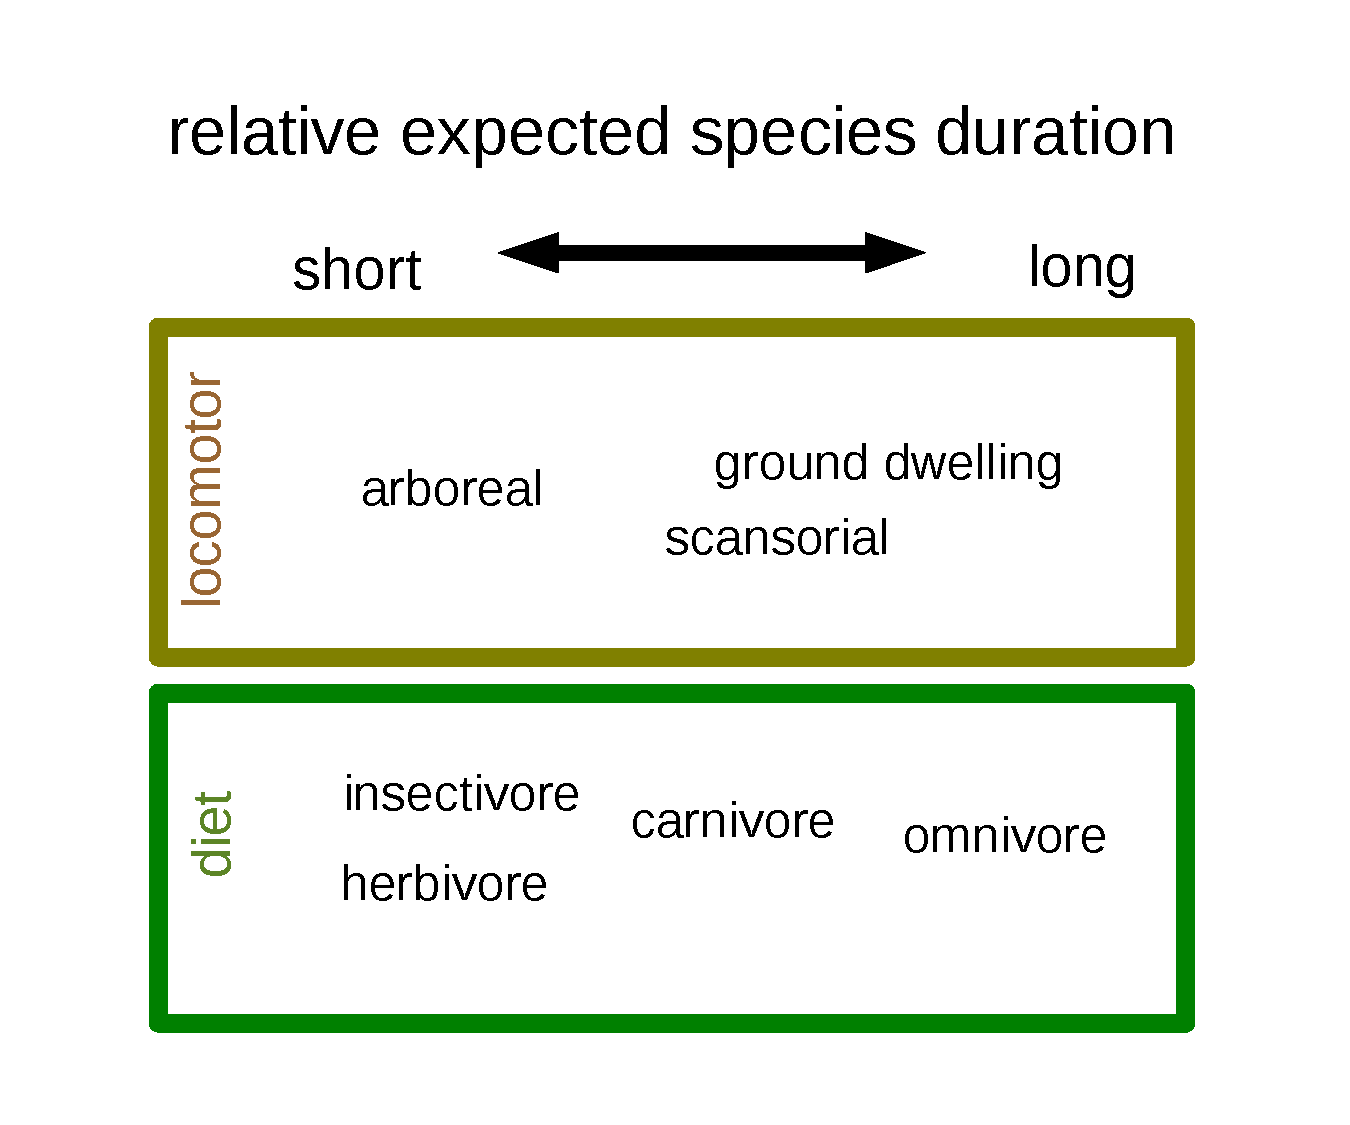
\includegraphics[height=0.8\textheight,width=\textwidth,keepaspectratio=true]{figure/smits_2015_results}
%  \end{center}
%
%  \attrib{\footnotesize{Smits, 2015, \em{PNAS}}}
%\end{frame}

\begin{frame}
  \frametitle{Conceptualizing the question and data}
  \begin{center}
    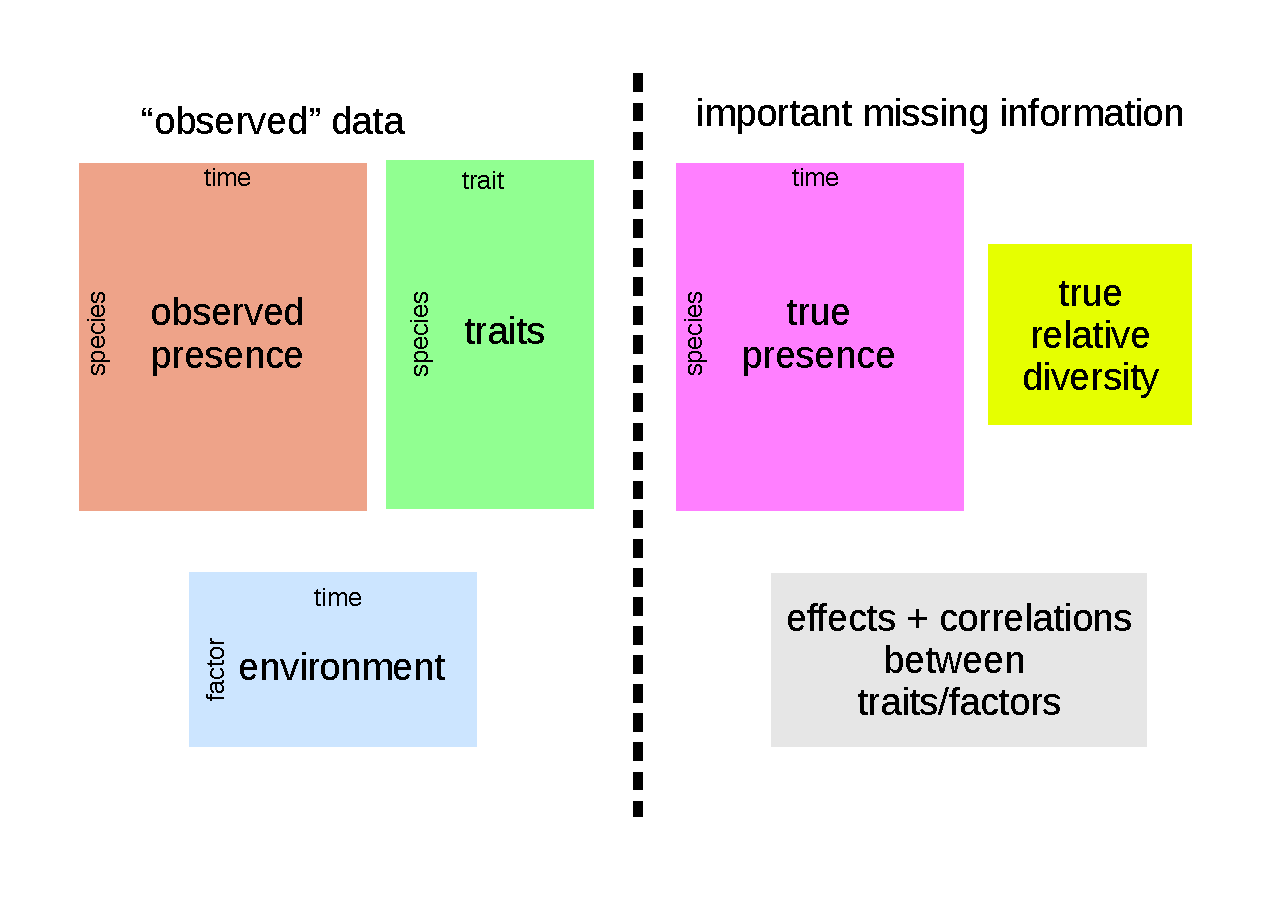
\includegraphics[width=\textwidth,height=\textheight,keepaspectratio=true]{figure/problem_concept}
  \end{center}
\end{frame}

\begin{frame}
  \frametitle{Conceptualizing the analysis}
  \begin{center}
    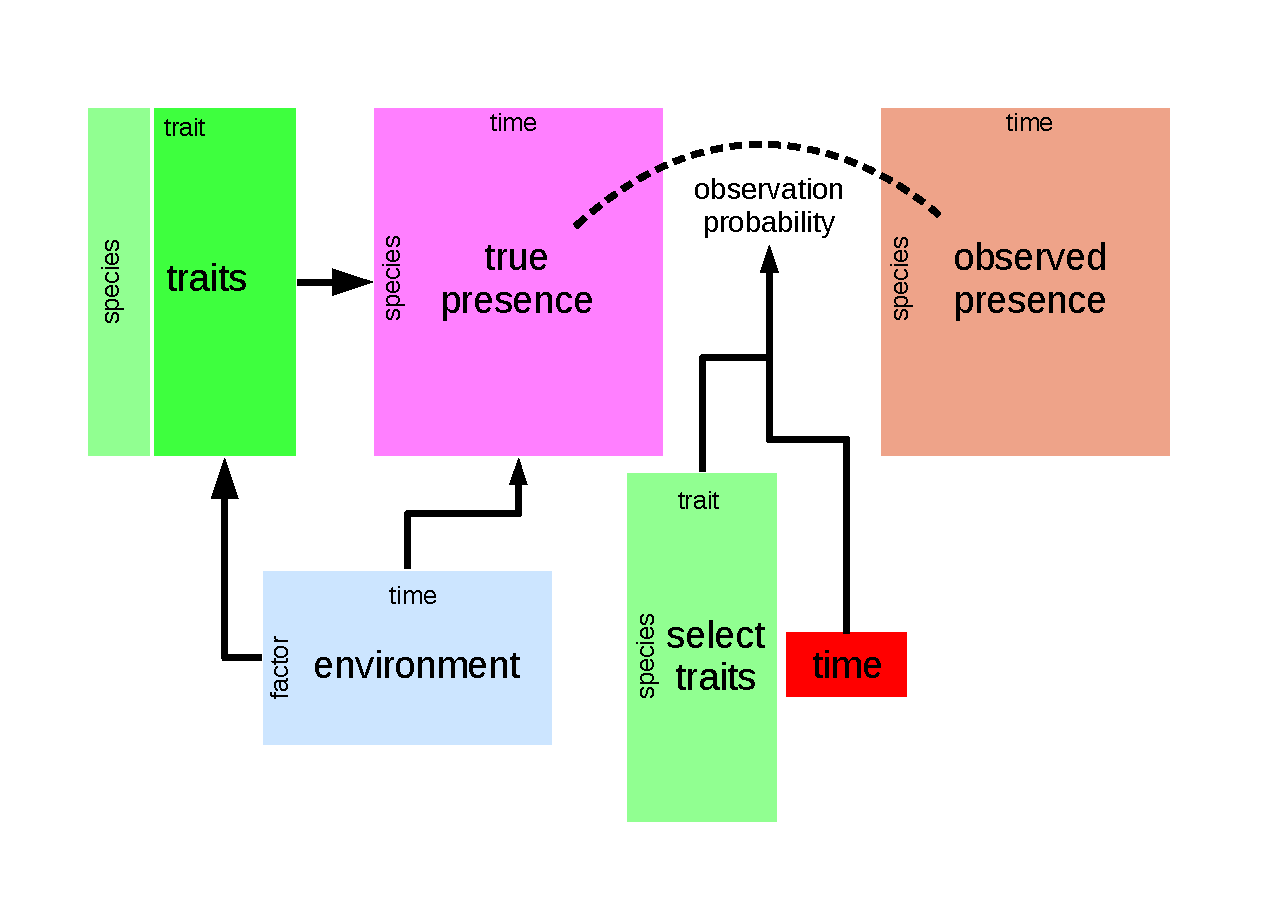
\includegraphics[width=\textwidth,height=\textheight,keepaspectratio=true]{figure/paleo_fourth_corner}
  \end{center}
\end{frame}


\begin{frame}
  \frametitle{Hidden Markov Model with absorbing state}
  \begin{block}{Jolly-Seber CMR/Restricted occupancy model}
    \begin{align*}
      y_{i, t} &\sim \text{Bernoulli}(z_{i, t} p_{i, t}) \\
      z_{i, t = 1} &\sim \text{Bernoulli}(\phi_{i, t = 1}) \\
      z_{i, t} &\sim \text{Bernoulli}\left(z_{i, t - 1} \pi_{i,t} + \sum_{x = 1}^{t}(1 - z_{i, x}) \phi_{i, t}\right)
    \end{align*}
    \begin{scriptsize}
      \(y\) observed state; \(z\) estimated state.

      \(p\) observation; \(\phi\) origination; \(\pi\) survival.

      \(i\) in \(N\); \(t\) in \(T\).
    \end{scriptsize}
  \end{block}
\end{frame}

\begin{frame}
  \frametitle{Modeling the probabilities; individual-level}
  \begin{block}{Multi-level logistic regression}
    \begin{align*}
      p_{i, t} &\sim \text{logit}^{-1}(b_{t} + e_{j[i]} + \beta^{p} mass_{i}) \\
      \phi_{i, t} &\sim \text{logit}^{-1}(f^{\phi}_{j[i], t} + o^{\phi}_{k[i]} + \beta^{\phi} mass_{i}) \\
      \pi_{i, t} &\sim \text{logit}^{-1}(f^{\pi}_{j[i], t} + o^{\pi}_{k[i]} + \beta^{\pi} mass_{i})
    \end{align*}
    \begin{scriptsize}
      observation: \(b_{t}\) time-varying intercept; \(e_{j[i]}\) functional group eff; \(\beta^{p}\) mass eff.
      
      origination: \(f^{\phi}_{j[i], t}\) time/FG-varying intercept; \(o^{\phi}_{j[i]}\) order eff; \(\beta^{\phi}\) mass eff.
      
      survival: \(f^{\pi}_{j[i], t}\) time/FG-varying intercept; \(o^{\pi}_{j[i]}\) order eff; \(\beta^{\pi}\) mass eff.
    \end{scriptsize}
  \end{block}
\end{frame}

%\gamma^{j = 1}_0 + \gamma^{j = 1}_1 phase_{2} + \gamma^{j = 1}_{2} phase_{3} + \gamma^{j = 1}_{3} temp_{t} \\
\begin{frame}
  \frametitle{Modeling the probabilities; group-level}
  \begin{block}{Multivariate regression of time/FG-varying intercept}
    \begin{align*}
      f^{\phi} &\sim \text{MVN}\left(
      \begin{matrix}
        U \gamma^{\phi}_{j = 1} \\
        %U_{t, \_} \gamma^{\phi}_{j = 2} \\
        \vdots \\
        U \gamma^{\phi}_{j = J}
      \end{matrix}, 
      \text{diag}(\tau_{f^{\phi}}) \Omega_{f^{\phi}} \text{diag}(\tau_{f^{\phi}}) \right) \\
      f^{\pi} &\sim \text{MVN}\left(
      \begin{matrix}
        U \gamma^{\pi}_{j = 1} \\
        %U_{t, \_} \gamma^{\pi}_{j = 2} \\
        \vdots \\
        U \gamma^{\pi}_{j = J}
      \end{matrix}, 
      \text{diag}(\tau_{f^{\pi}}) \Omega_{f^{\pi}} \text{diag}(\tau_{f^{\pi}}) \right)
    \end{align*}
    \begin{scriptsize}
      \(U\) matrix group-level covariates; \(\gamma^{\phi}\), \(\gamma^{\pi}\) vectors group-level reg coefs.
      
      \(\Omega_{\phi}\), \(\Omega_{\pi}\) corr matrix of FG by time; \(\tau_{\phi}\), \(\tau^{\pi}\) scale of FG by time.
    \end{scriptsize}
  \end{block}
\end{frame}


\begin{frame}
  \frametitle{Final details (priors, implementation)}
  \begin{itemize}
    \item Random-walk priors for time-varying intercepts to control.
    \item Strong priors against effects of mass on observation, origination, survival (e.g. \(\mathcal{N}(0, 0.5)\)).
    \item Strong priors against effects of group-level covariates on observation, origination, survival (e.g. \(\mathcal{N}(0, 0.5)\)).
    \item Strong prior against correlations between functional groups over time (e.g. LKJ\((4)\)).
    \item Programmed as marginalization problem b/c gradient based estimation.
  \end{itemize}
\end{frame}


\begin{frame}
  \frametitle{Parameter estimation and inference}
  \begin{columns}
    \begin{column}{0.45\textwidth}
      \begin{itemize}
        \item full HMC/MCMC slow
        \item \textbf{Automatic Differentiation Variational Inference (ADVI)}
          \begin{itemize}
            \item approximate Bayesian inference
            \item assumes posterior is Gaussian, no correlation between parameters
            \item true Bayesian posterior
          \end{itemize}
      \end{itemize}
    \end{column}
    \begin{column}{0.55\textwidth}
      
\includegraphics[height=0.9\textheight,width=\textwidth,keepaspectratio=true]{figure/stan_logo}
    \end{column}
  \end{columns}
\end{frame}


\begin{frame}
  \frametitle{Model adequate? Posterior predictive check}
  \begin{center}
    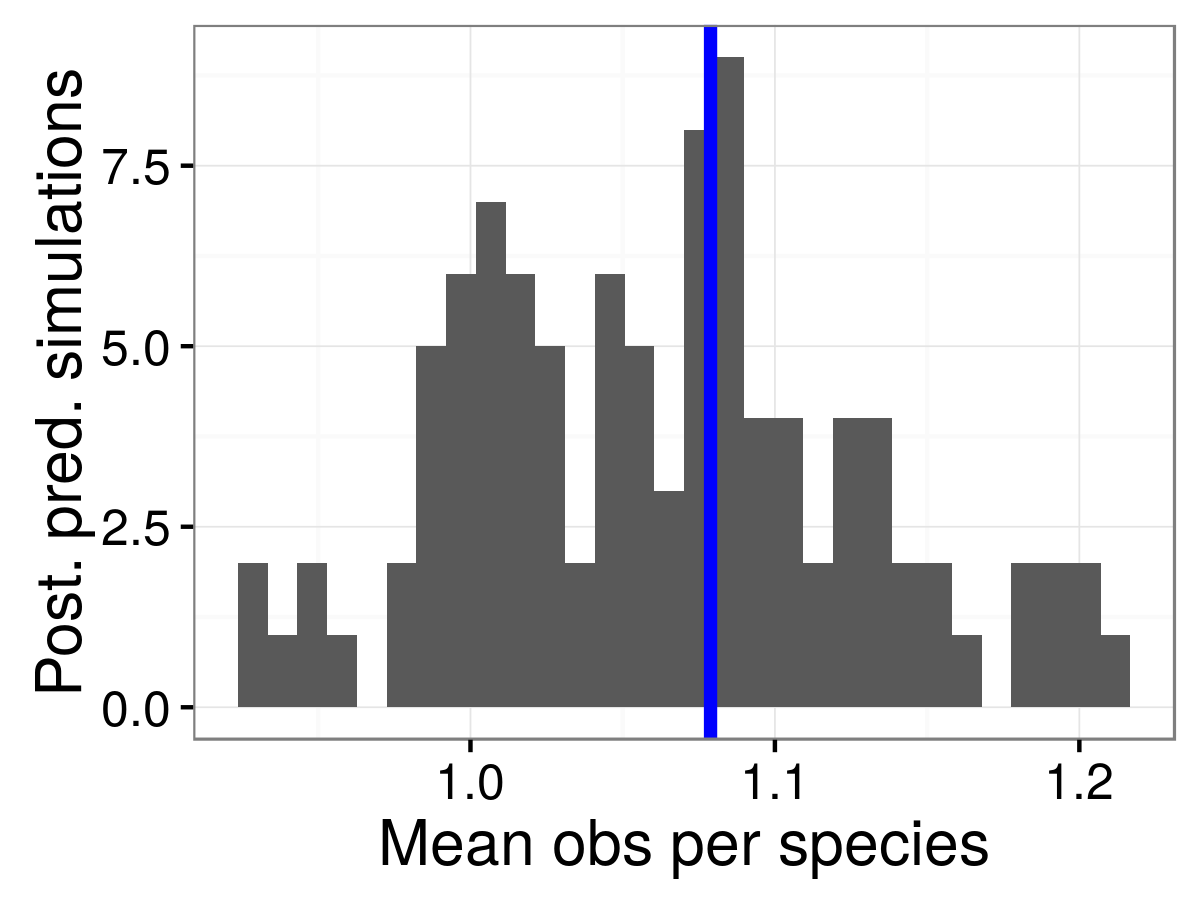
\includegraphics[height=0.8\textheight,width=\textwidth,keepaspectratio=true]{figure/pred_occ_bd}
  \end{center}
\end{frame}

\begin{frame}
  \frametitle{Observation probability; NALMA}
  \begin{center}
    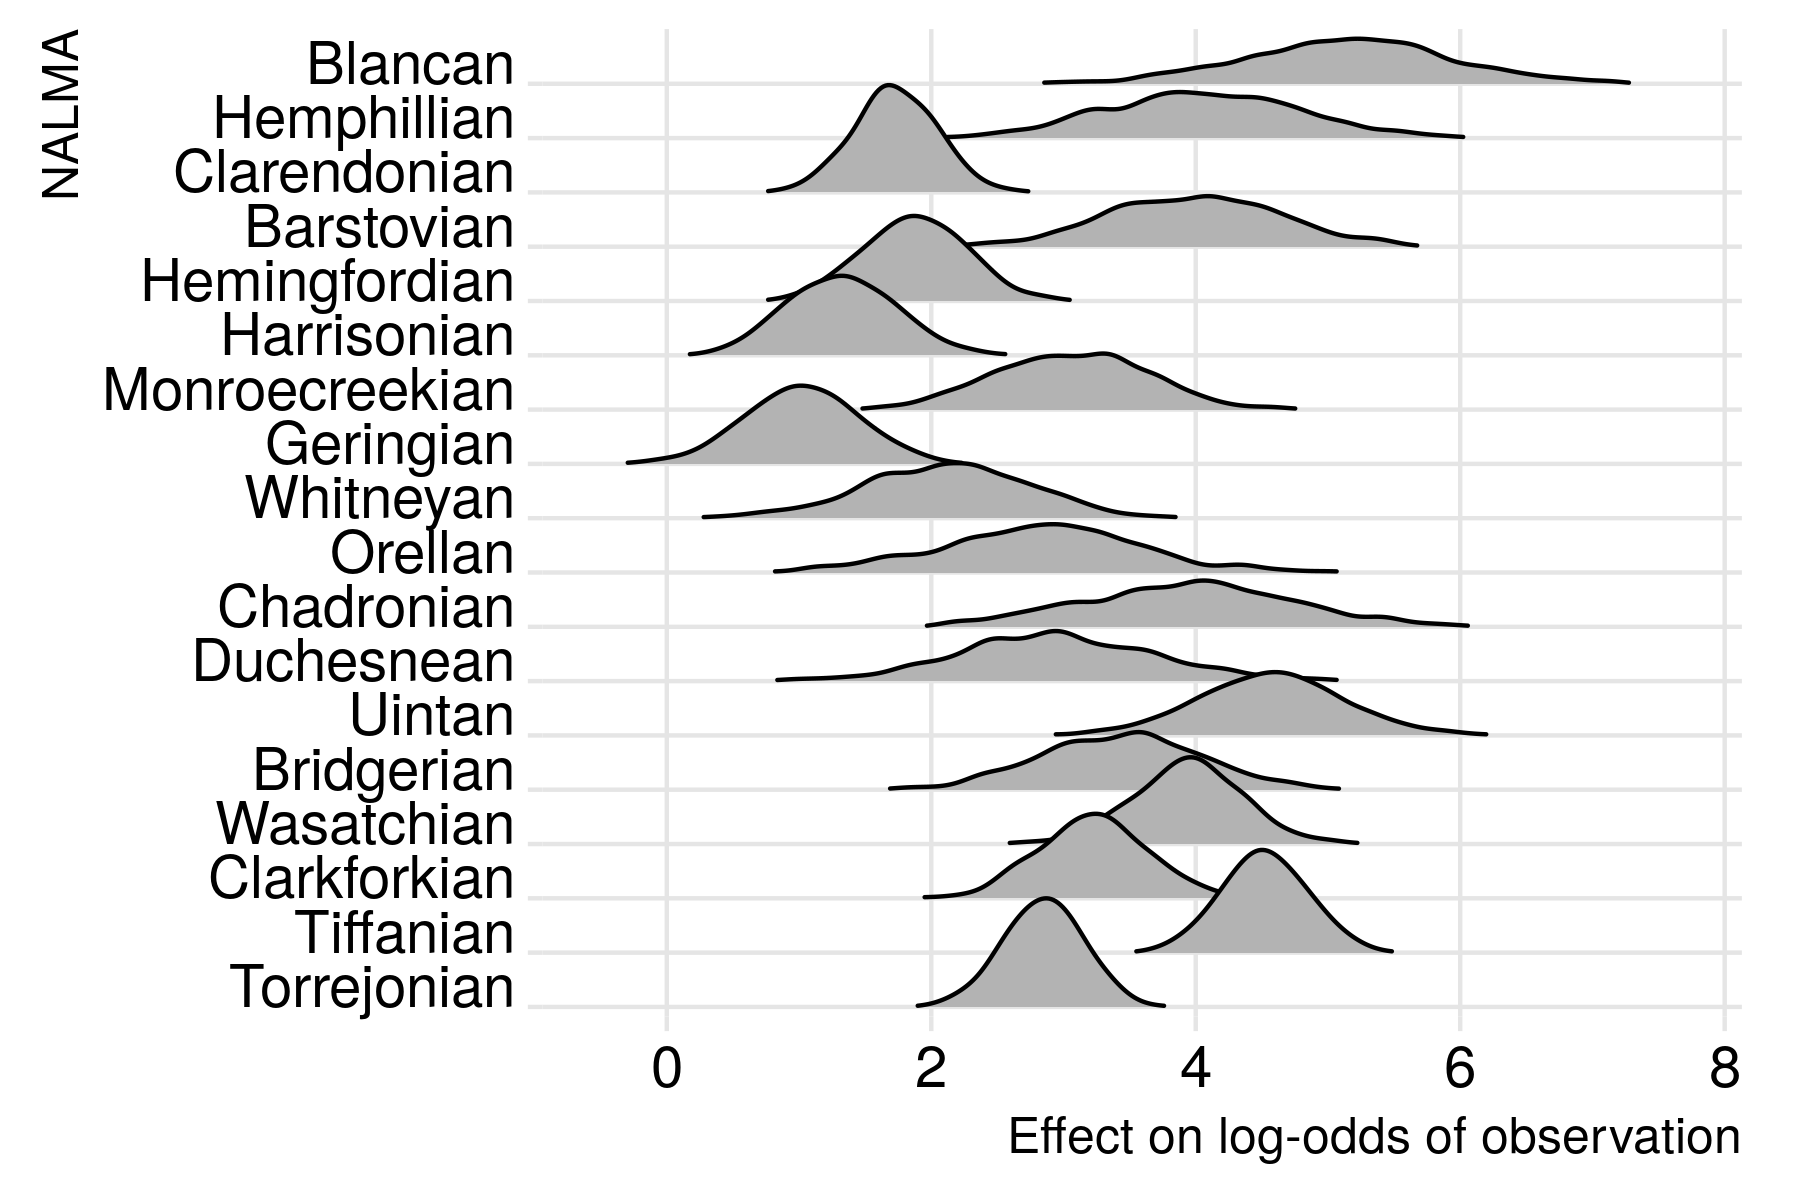
\includegraphics[height=0.8\textheight,width=\textwidth,keepaspectratio=true]{figure/time_observation}
  \end{center}
\end{frame}

\begin{frame}
  \frametitle{Observation probability; functional group}
  \begin{center}
    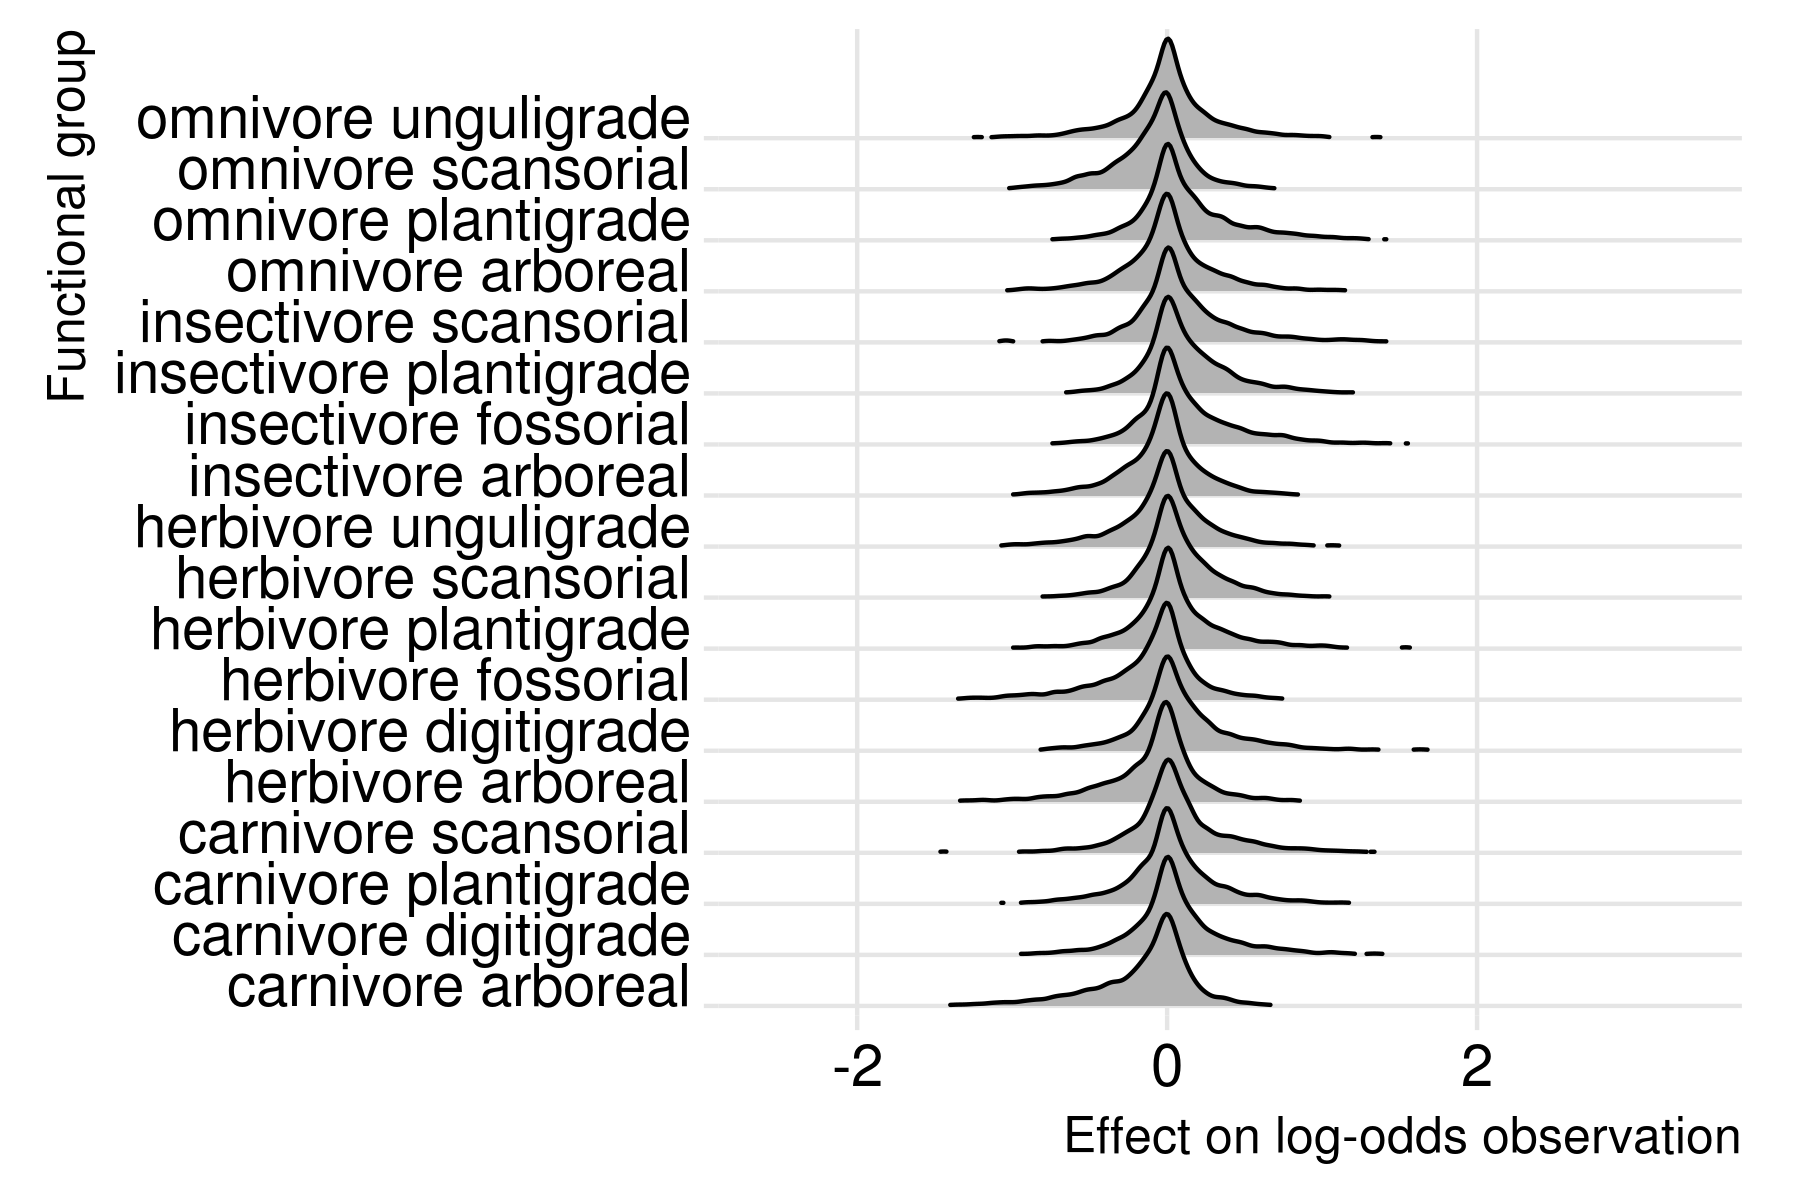
\includegraphics[height=0.8\textheight,width=\textwidth,keepaspectratio=true]{figure/ecotype_observation}
  \end{center}
\end{frame}

\begin{frame}
  \frametitle{Origination probability; individual-level}
  \begin{center}
    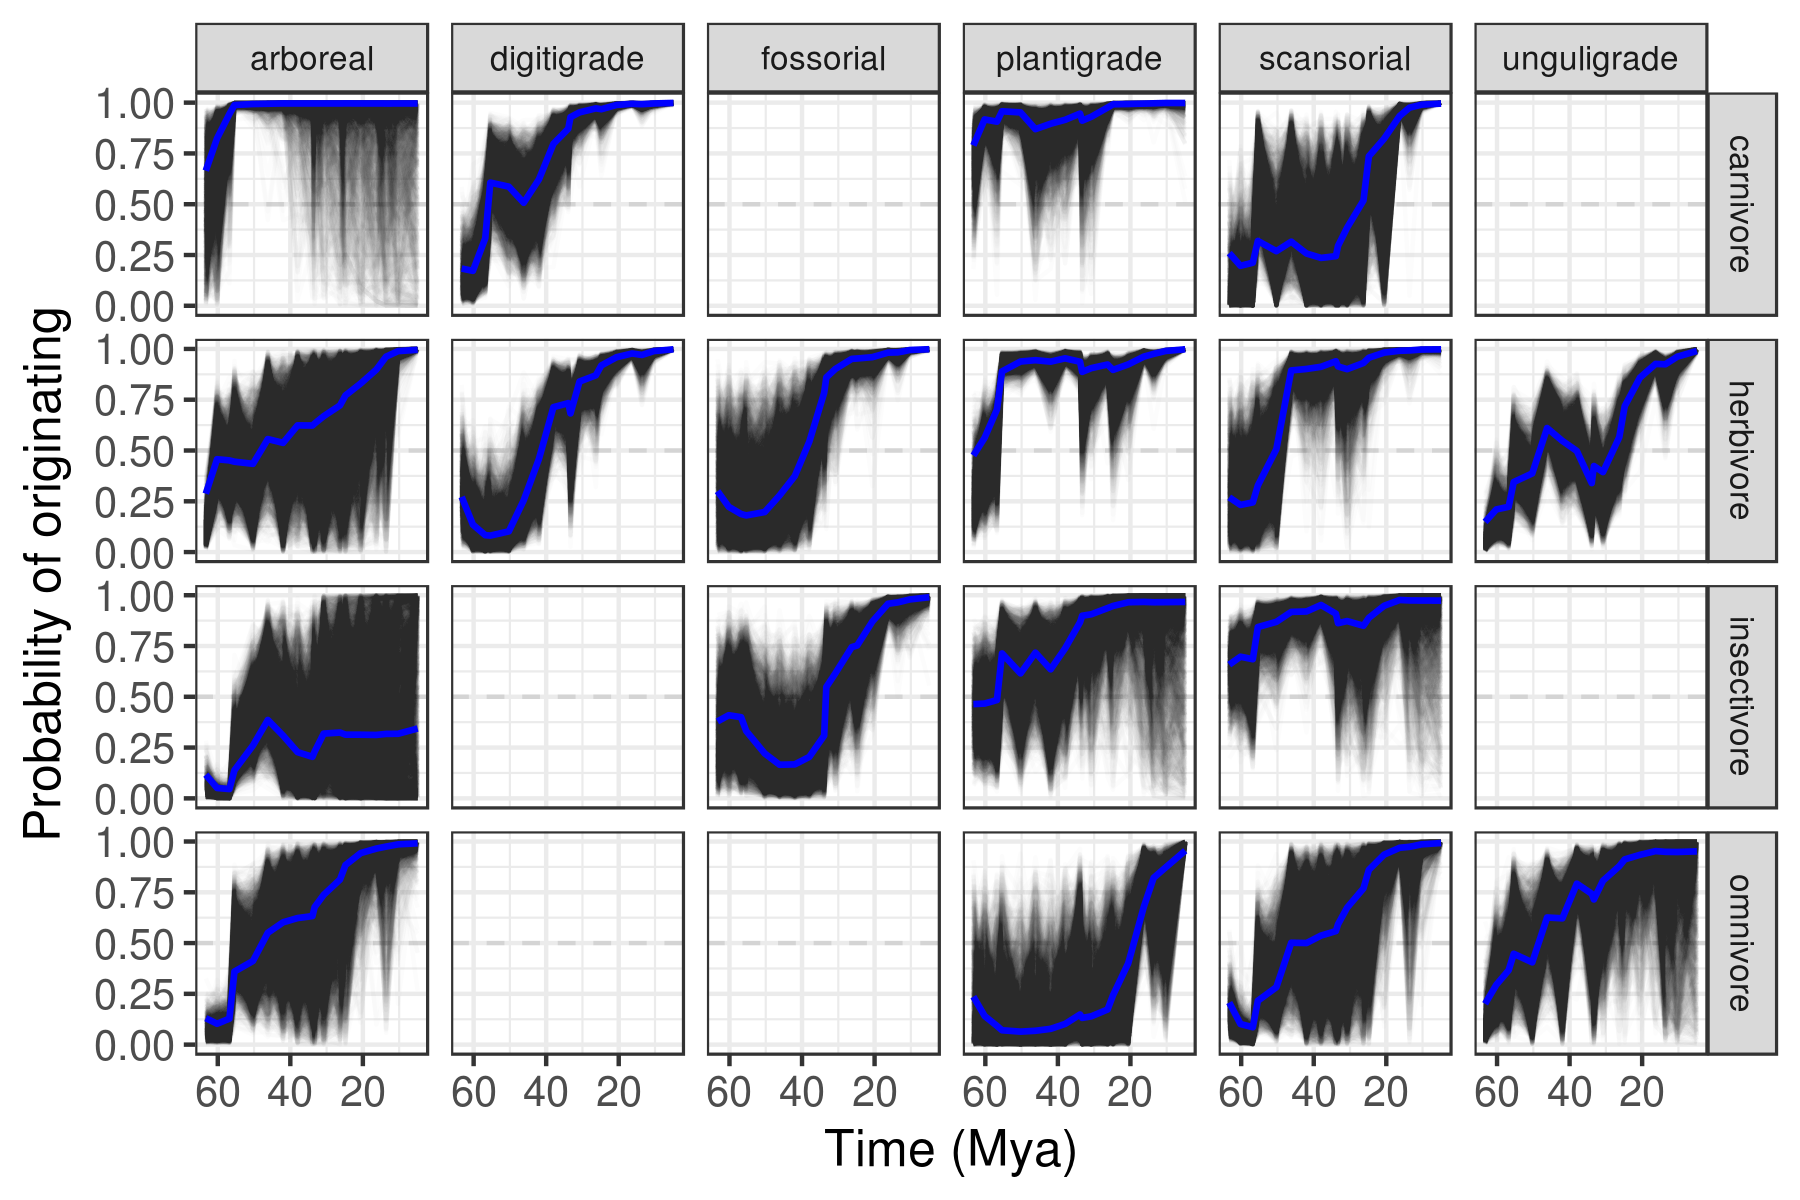
\includegraphics[height=0.8\textheight,width=\textwidth,keepaspectratio=true]{figure/ecotype_origin_bd}
  \end{center}
\end{frame}

\begin{frame}
  \frametitle{Origination probability; group-level}
  \begin{center}
    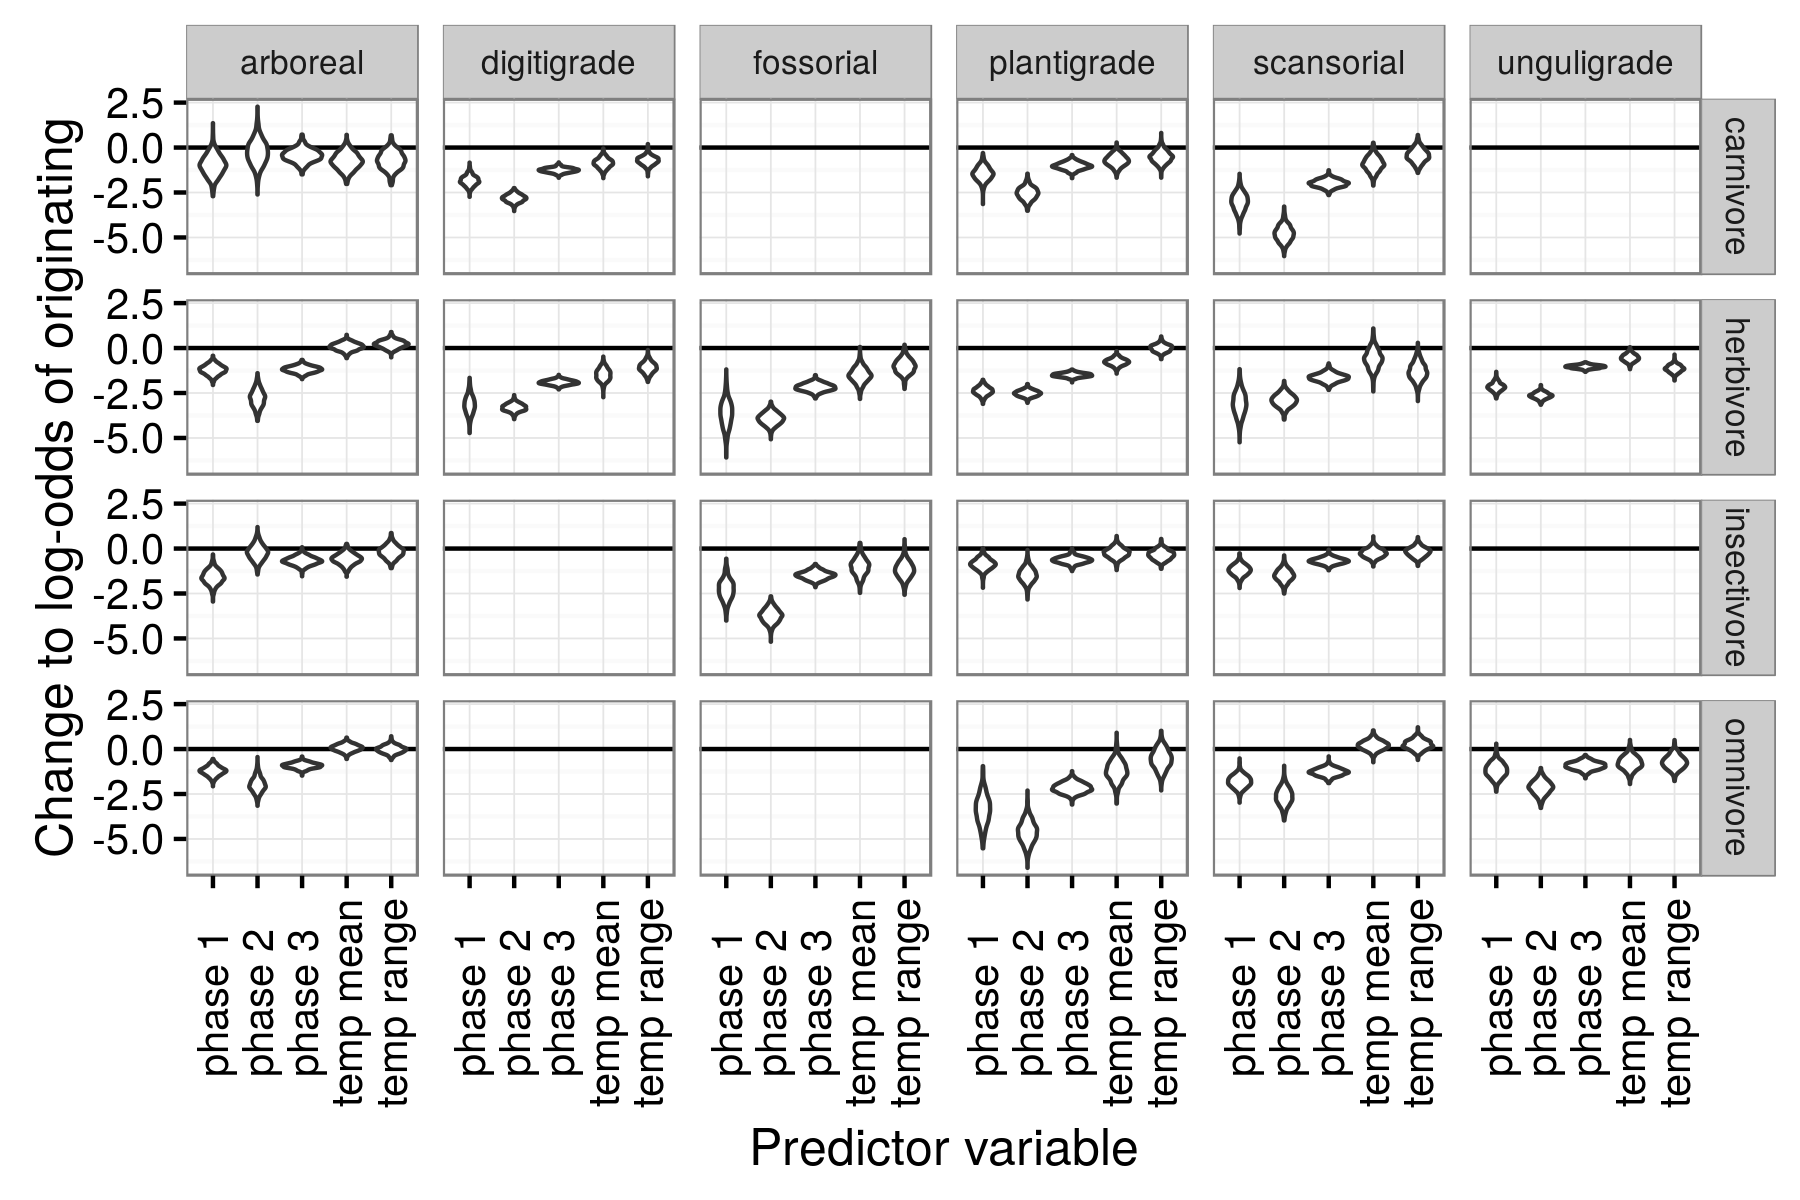
\includegraphics[height=0.8\textheight,width=\textwidth,keepaspectratio=true]{figure/group_on_origin_bd}
  \end{center}
\end{frame}

%\begin{frame}
%  \frametitle{Origination probability; correlation between FG}
%  \begin{center}
%    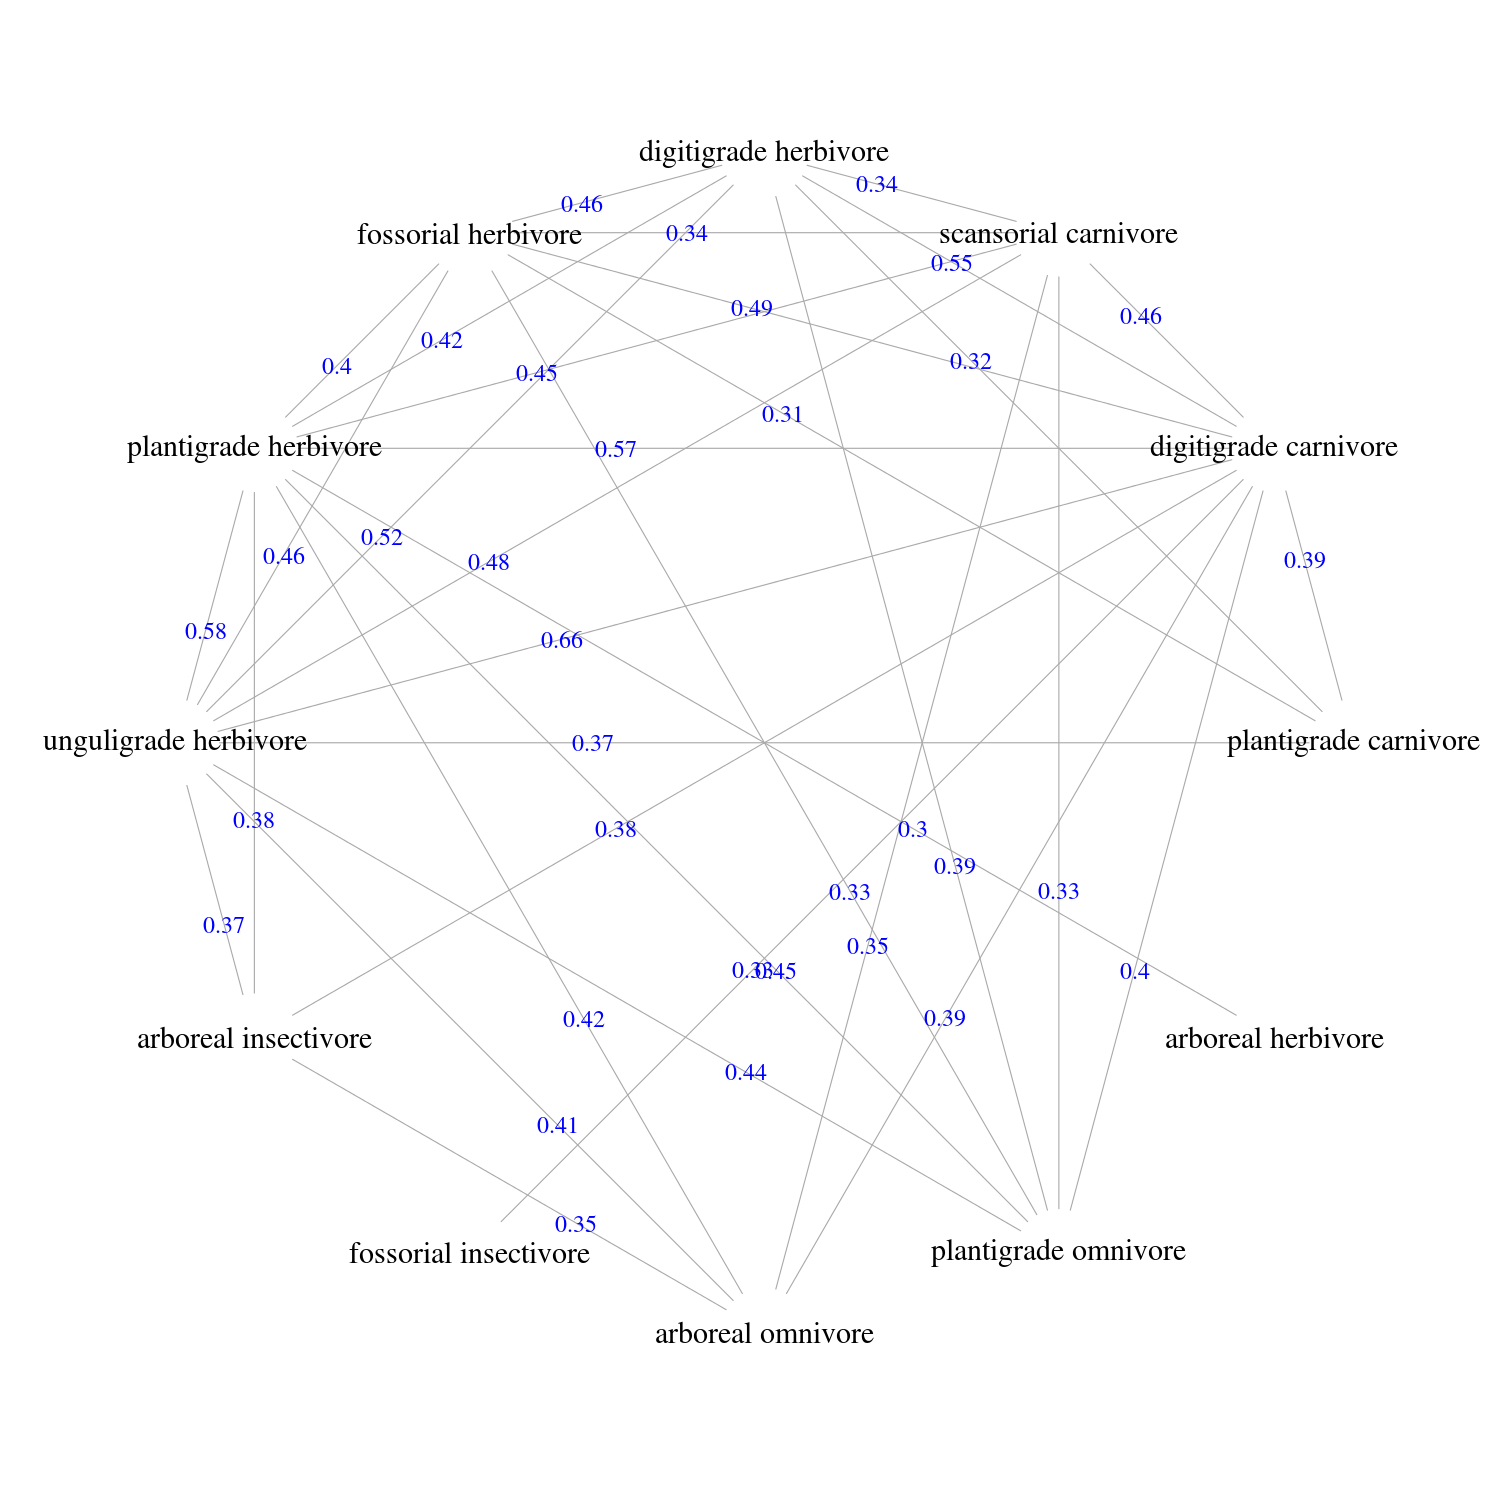
\includegraphics[height=0.8\textheight,width=\textwidth,keepaspectratio=true]{figure/origin_sig_corr}
%  \end{center}
%\end{frame}

\begin{frame}
  \frametitle{Survival probability; individual-level}
  \begin{center}
    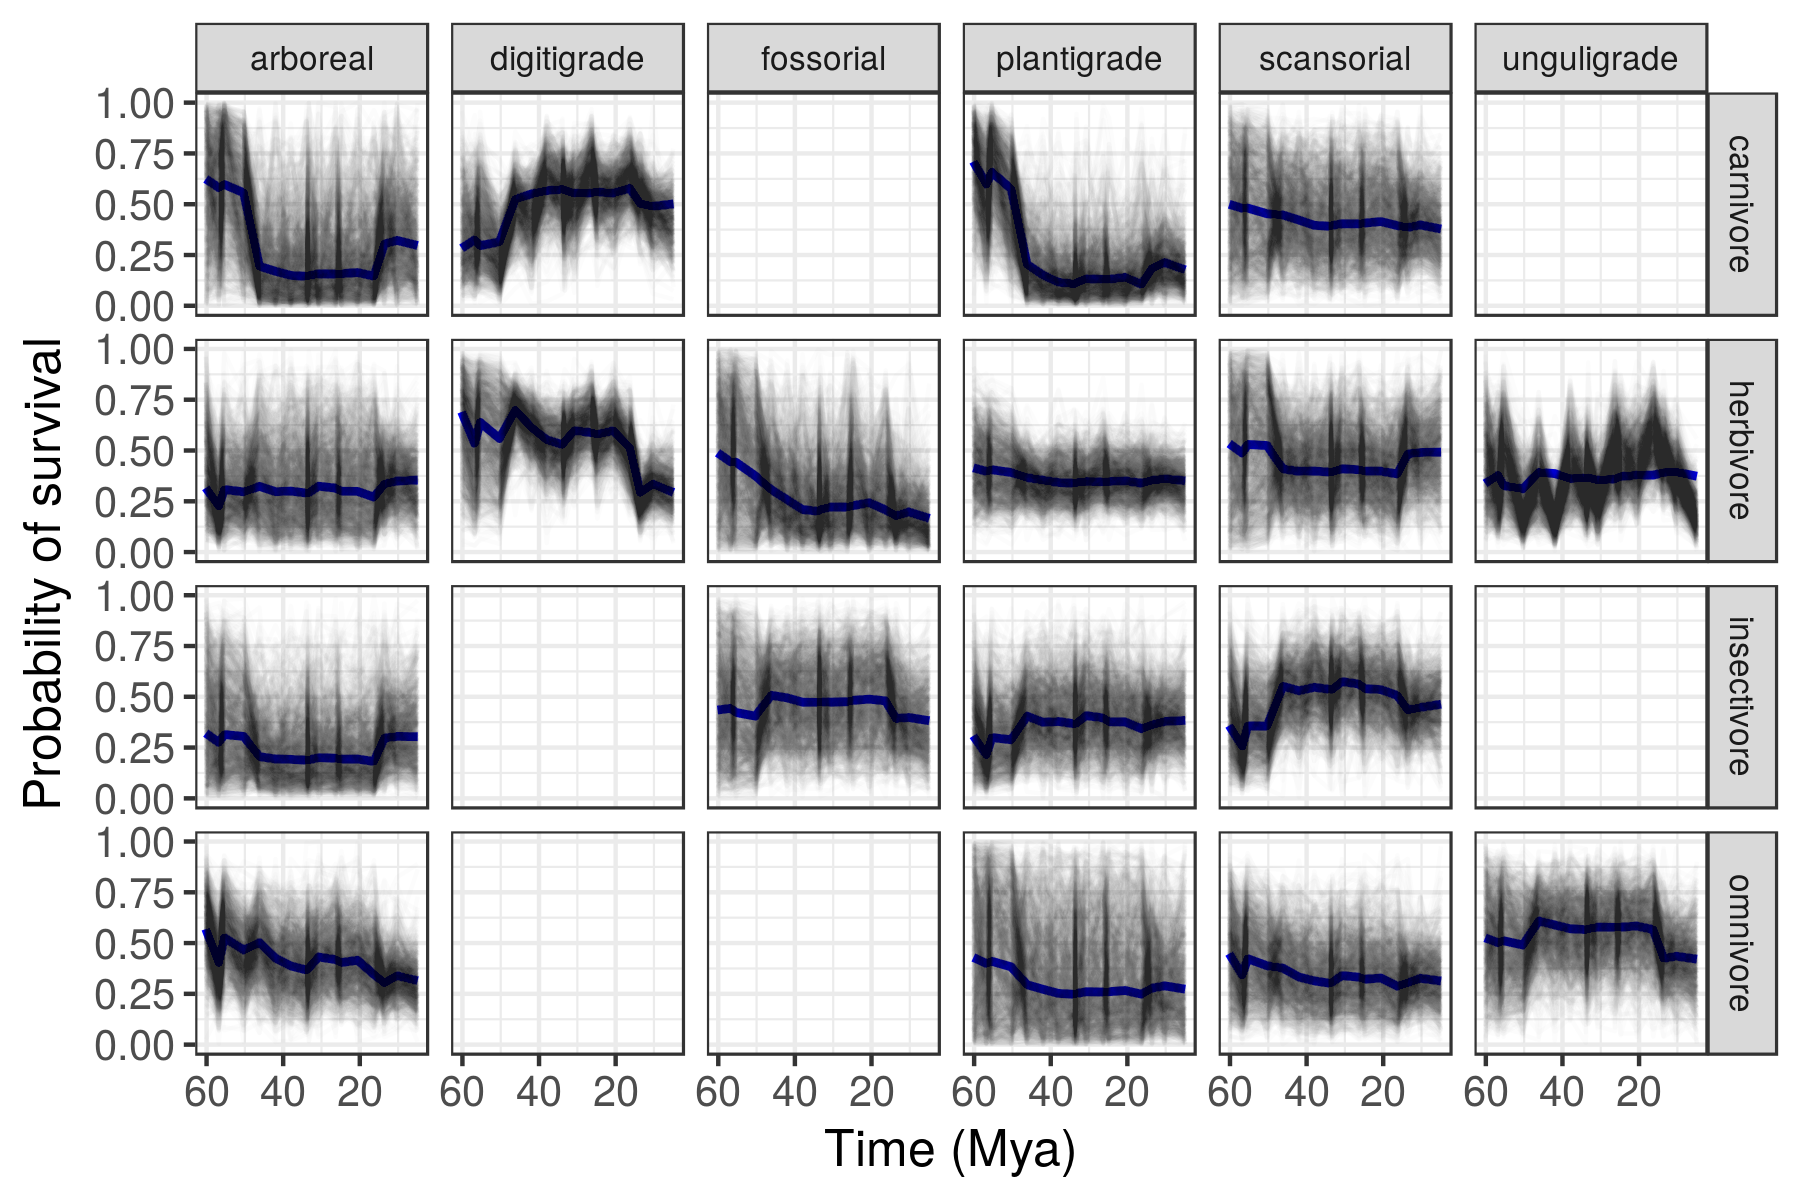
\includegraphics[height=0.8\textheight,width=\textwidth,keepaspectratio=true]{figure/ecotype_survival_bd}
  \end{center}
\end{frame}

\begin{frame}
  \frametitle{Survival probability; group-level}
  \begin{center}
    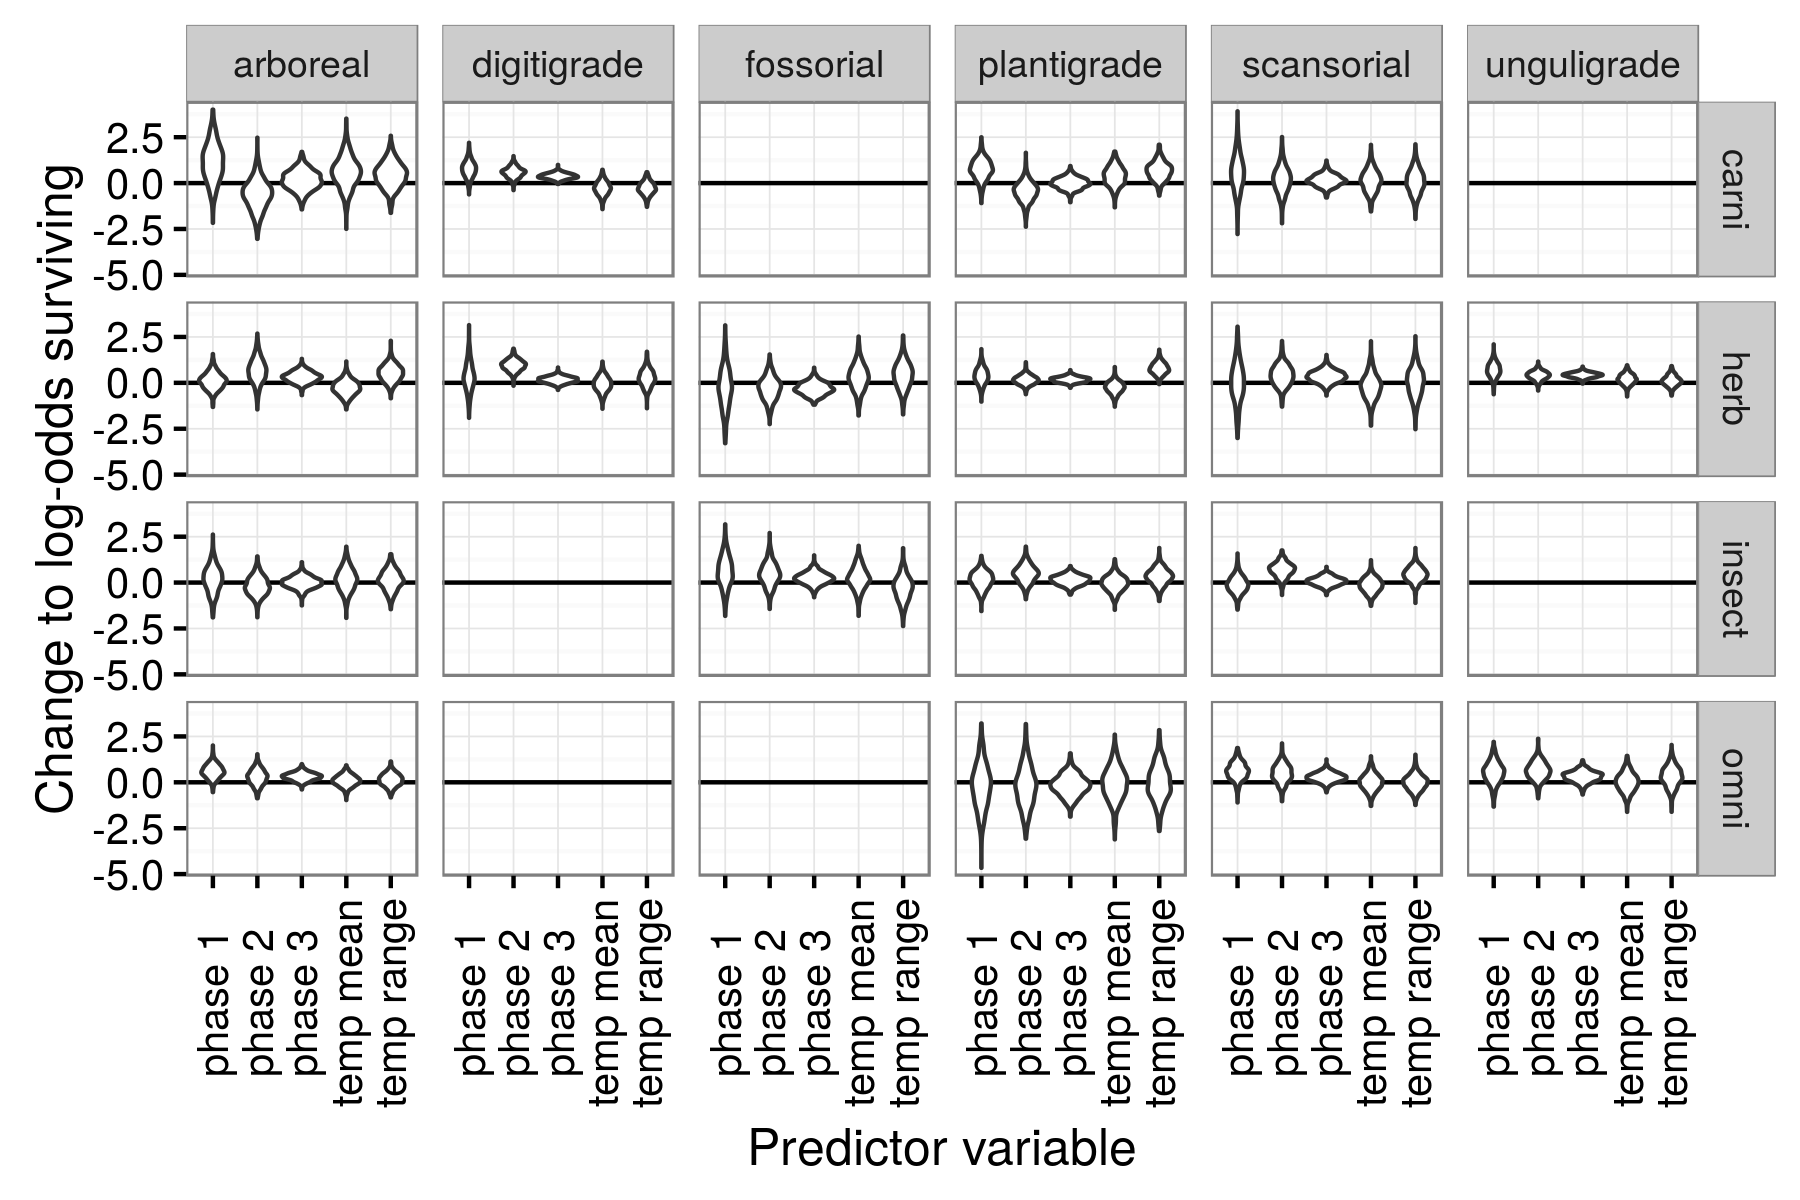
\includegraphics[height=0.8\textheight,width=\textwidth,keepaspectratio=true]{figure/group_on_survival_bd}
  \end{center}
\end{frame}

\begin{frame}
  \frametitle{Standing diversity of functional groups through time}
  \begin{center}
    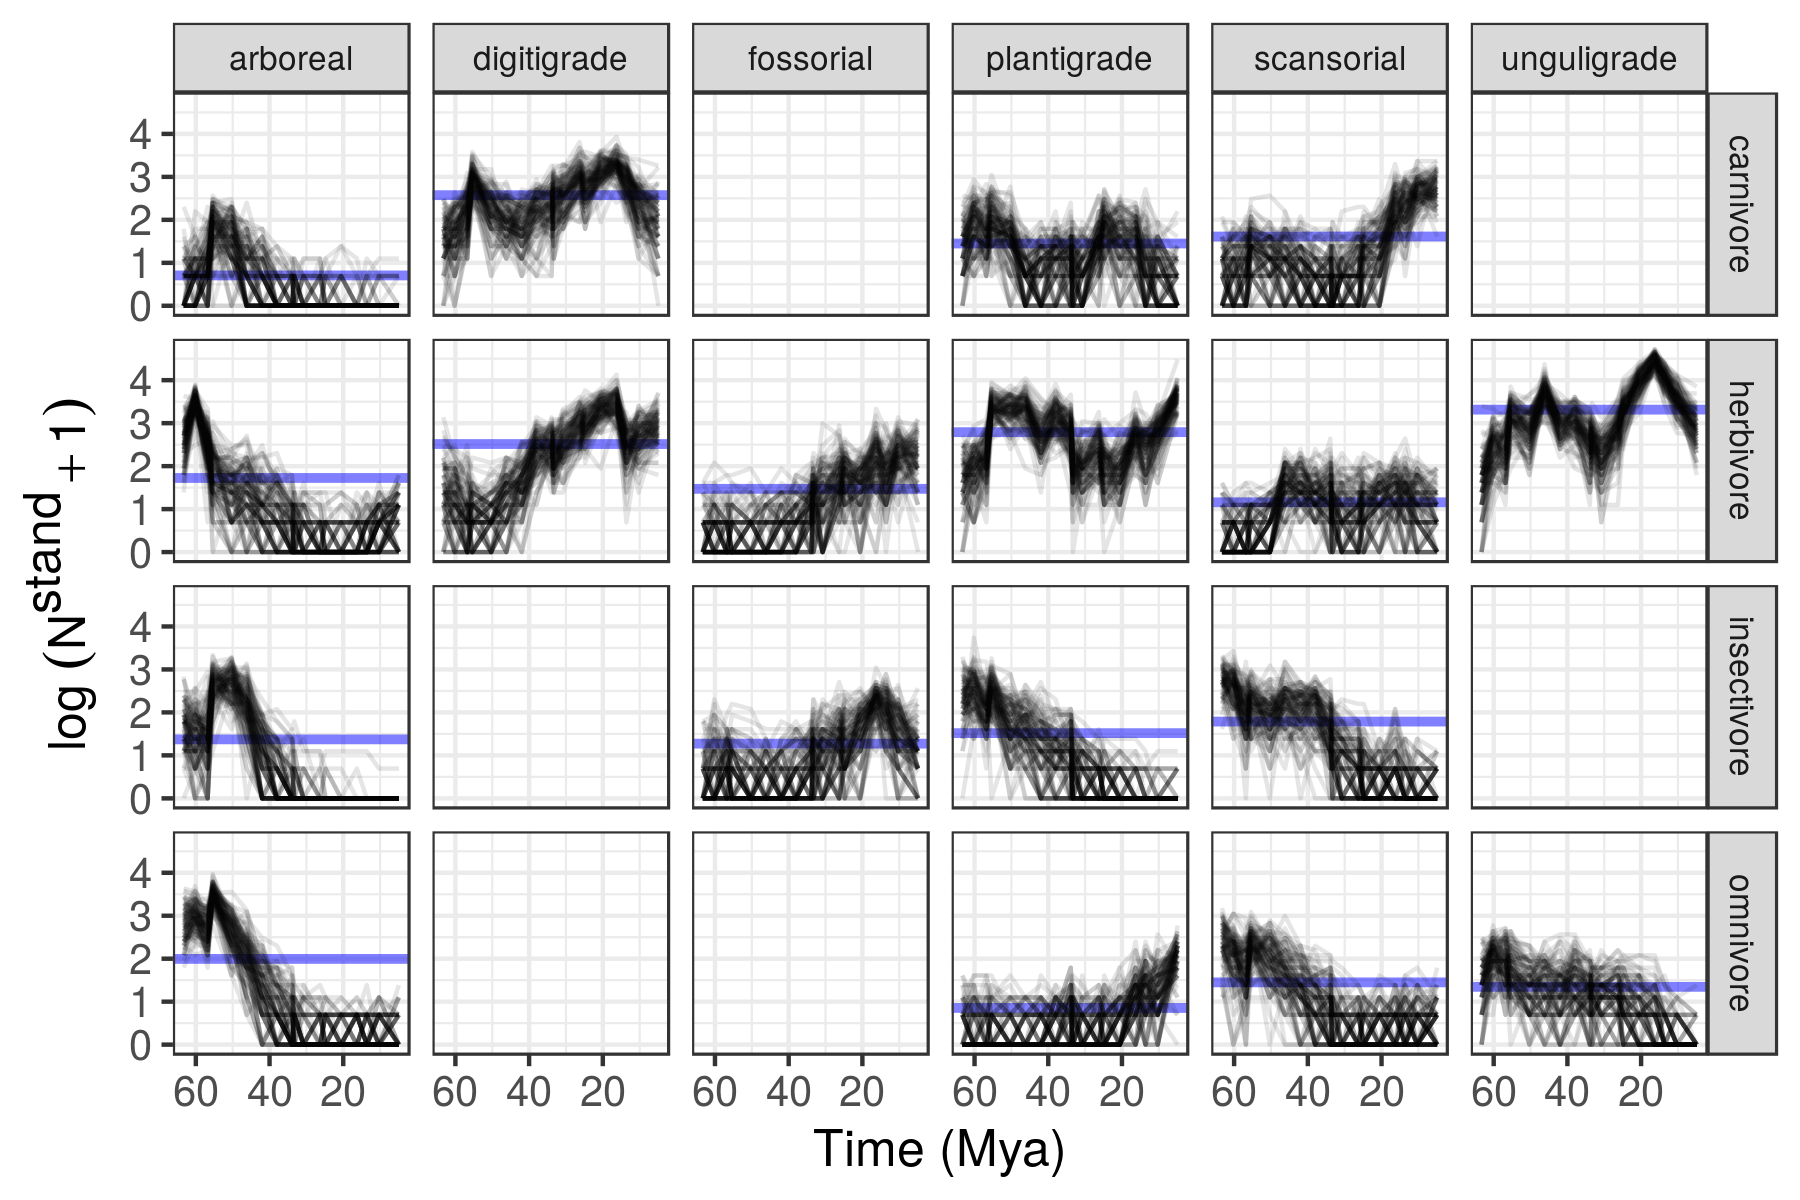
\includegraphics[height=0.8\textheight,width=\textwidth,keepaspectratio=true]{figure/ecotype_diversity}
  \end{center}
\end{frame}

\begin{frame}
  \frametitle{Relative diversity of functional groups through time}
  \begin{center}
    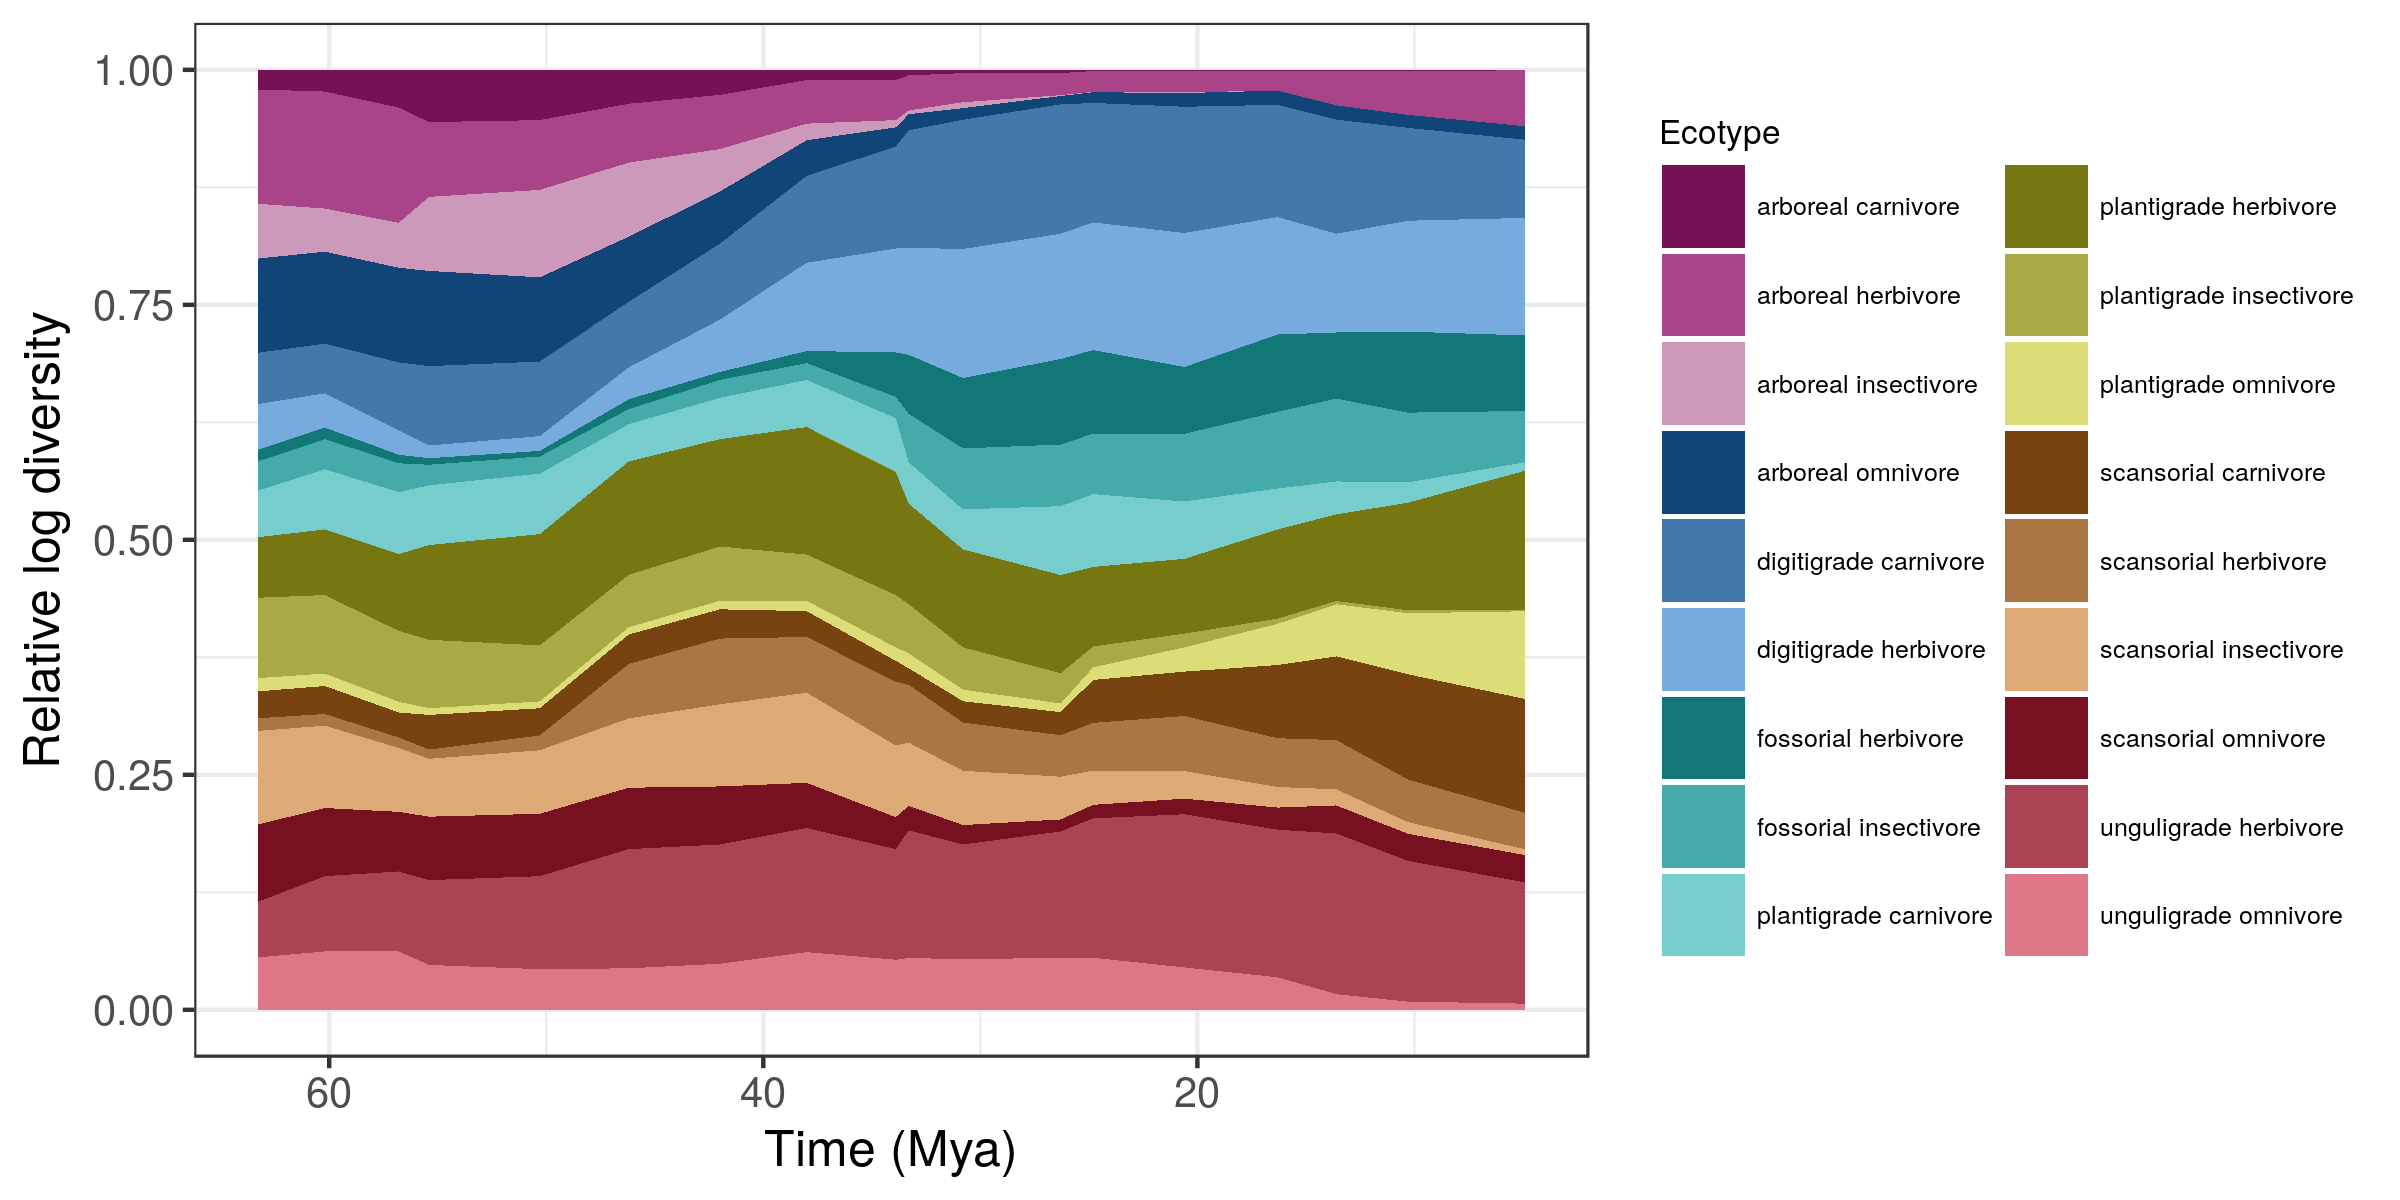
\includegraphics[height=0.8\textheight,width=\textwidth,keepaspectratio=true]{figure/relative_diversity}
  \end{center}
\end{frame}


\begin{frame}
  \begin{block}{Changes to relative diversity between Neogene/Paleogene}
    \begin{itemize}
      \item \alert{increase}
        \begin{itemize}
          \item digitigrade, plantigrade, unguligrade herbivores
          \item fossorial functional groups
          \item plantigrade omnivores
        \end{itemize}
      \item \alert{decrease}
        \begin{itemize}
          \item near total loss of arboreal functional groups
          \item plantigrade, scansorial insectivores
          \item unguligrade omnivores
        \end{itemize}
    \end{itemize}
  \end{block}
\end{frame}

\begin{frame}
  \begin{block}{Conclusions}
  \end{block}
\end{frame}


\begin{frame}
  \frametitle{Acknowledgements}
  \begin{columns}
    \begin{column}{0.5\textwidth}
      \begin{itemize}
        \item UC Berkeley
          \begin{itemize}
            \item \textbf{Seth Finnegan}, \\Adiel Klompmaker, \\Emily Orzechowski, \\Larry Taylor, \\Sara Kahanamoku, \\Josh Zimmt
          \end{itemize}
        \item UChicago
          \begin{itemize}
            \item \textbf{Kenneth D. Angielczyk}, \\\textbf{Michael J. Foote}, \\P. David Polly, \\Richard H. Ree, \\Graham Slater
          \end{itemize}
      \end{itemize}
    \end{column}
    \begin{column}{0.5\textwidth}
      \begin{center}
        
\includegraphics[height=0.2\textheight,width=0.5\textwidth,keepaspectratio=true]{figure/twitter} 

        @PeterDSmits
      \end{center}
      \vspace*{0.05\textheight}
      \begin{center}
        
\includegraphics[height=0.4\textheight,width=\textwidth,keepaspectratio=true]{figure/paleodb}
      \end{center}
    \end{column}
  \end{columns}
\end{frame}

\end{document}
